\documentclass{beamer}
\usetheme{Frankfurt}

\usepackage{graphicx}

\usepackage{url}

\usepackage{color}

\title{The Search for a Universal Turing Machine}
\author{Steven Dee, Justin Gray, Josh Lee, Neil Sandberg}
\date{\today}

\begin{document}

\frame{\titlepage}

\section[Outline]{}
\frame{
	\frametitle{Overview}
	\tableofcontents
}

\section{Overall Objectives}
\frame{
	\frametitle{Overall Objectives}
	Can we use the discovery of Universal Turing Machines as an analogy for the evolution of complex organisms? 
	\begin{columns}
		\begin{column}{.75\textwidth}
			\begin{itemize}
				\item Test the possibility of discovering a set of Universal Turing Machines via a Genetic Algorithm optimization
				\item Create a web application to publish the results of the optimization
					\begin{itemize}
						\item Real-time link to database being populated by optimization results
					\end{itemize}
			\end{itemize}
		\end{column}
		\begin{column}{.25\textwidth}
			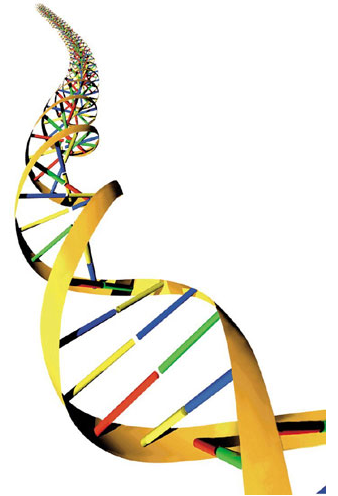
\includegraphics[width=\textwidth]{images/dna.png}
		\end{column}
	\end{columns}
}

\section{Genetic Algorithm}
\frame{
	\frametitle{Genetic Algorithm}
	{\bf Genetic Algorithm Structure}: 
	The genetic algorithm is comprised of the following key parts
	\begin{itemize}
		\item Turing Machine Encoding
		\item Fitness Evaluation
			\begin{itemize}
				\item Constant input
				\item Random input
				\item Input with generational drift
			\end{itemize}
		\item Mutation Algorithm
		\item Parent Selection and Reproduction Algorithms
	\end{itemize}
}

\subsection{Turing Machine Encoding}
\frame{
	\frametitle{Turing Machine Encoding}
	Binary string encoding selected \\
	Example: '111110101001100101000110', 3 State Turing Machine
	\begin{enumerate}
		\item Break encoding into individual genes: \\
		1111  1010  1001  1001  0100  0110
		\item Each Gene is one entry in a state transition table: 1111\\
		next state: 11 --- 3; write bit: 1; movement: 1 --- Right
		\item State transition table for example 3-state TM
	\end{enumerate}

	\begin{table}
		\begin{tabular}{|c|c||c|c|c|} \hline
		{\bf current state} & {\bf read bit} & {\bf next state} & {\bf write bit} & {\bf movement} \\ \hline
		1 & 0 & 11 & 1 & 1\\ \hline
		1 & 1 & 10 & 1 & 0\\ \hline
		2 & 0 & 10 & 0 & 1\\ \hline
		2 & 1 & 10 & 0 & 1\\ \hline
		3 & 0 & 01 & 0 & 1\\ \hline
		3 & 1 & 01 & 1 & 1\\ \hline
		\end{tabular}
		\label{tab:example_TM}
	\end{table}

	
}
\subsection{Fitness Evaluation}
\frame{
	\frametitle{Fitness Evaluation}	
	Using a measure of complexity of TM output as fitness --- size of the compressed output of a TM. 
	\begin{itemize}
		\item 0000000000000000000000000 --- fitness: 11
		\item 1010101010101010101010101 --- fitness: 12
		\item 1011011010010101101010100 --- fitness: 20
	\end{itemize}
	deflate compression is used because it is lossless
	
	{\bf Input given to generate output:}
	\begin{itemize}
		\item constant input: the same input (in this case no input) is given to every generation
		\item random input: each generation a completely random input is created
		\item drifting input: each generation uses a 'mutated' input relative to the last generation
	\end{itemize}
}
\subsection{Mutation Algorithm}
\frame{
	\frametitle{Mutation Algorithm}
	30\% chance of mutation occurring with bit swapping method: \\
	Example: '111110101001100101000110', 3 State Turing Machine 
	\begin{itemize}
		\item 111110 {\bf 10} 10011001 {\bf 01} 000 {\bf 11} 0
		\item 111110 {\bf 01} 10011001 {\bf 10} 000 {\bf 11} 0
		\item 111110011001100110000110
	\end{itemize}
	Notice that three separate bit swaps occurred\\
	One of the bit swaps resulted in not actual change in the encoded information
	
	{\bf Key Parameters:}
	\begin{itemize}
		\item mutation rate: percentage of population that will undergo a mutation
		\item mutation frequency: average number of bit swaps that happen per mutation
	\end{itemize}
}
\subsection{Parent Selection and Reproduction}
\frame{
	\frametitle{Parent Selection and Reproduction}
	{\bf Parent Selection Method: Competition}
	\begin{itemize}
		\item small competitions are set up between randomly selected population members, the highest fitness wins
		\item each competitor is chosen from the whole population
		\item {\bf Key Parameter:} competition size determines selectiveness of the reproduction. Smaller competitions are less selective
	\end{itemize}
	\begin{columns}
		\begin{column}{.25\textwidth}
			\includegraphics[width=\textwidth]{images/init_population} 
		\end{column}
		\begin{column}{.25\textwidth}
			\includegraphics[width=\textwidth]{images/comp1} 
		\end{column}
		\begin{column}{.25\textwidth}
			\includegraphics[width=\textwidth]{images/comp2} 
		\end{column}
		\begin{column}{.25\textwidth}
			\includegraphics[width=\textwidth]{images/comp3} 
		\end{column}
	\end{columns}
}
\frame{
	\frametitle{Parent Selection and Reproduction}
	{\bf Reproduction Method: Crossover}
	\begin{itemize}
		\item Using a simple two-point cross over method
		\item cross overs only occur at gene boundaries in encoding
	\end{itemize}
	Example: \textcolor{red}{'111110101001100101000110'} and \textcolor{blue}{'101001011111101101001100'}
	\begin{enumerate}
		\item randomly pick cross over point: between 2nd gene and 4th gene
		\item cut parent encodings: 
			\begin{itemize}
				\item \textcolor{red}{1111---101010011001---01000110}
				\item \textcolor{blue}{1010---010111111011---01001100}
			\end{itemize}
		\item splice child from parent cuts: \textcolor{blue}{1010}---\textcolor{red}{101010011001}---\textcolor{blue}{01001100}
		\item final child: 101010101001100101001100
	\end{enumerate}
}

\section{Web Visualization App}
\frame{
	\frametitle{Web Visualization App}
	The purpose of this web app is to provide a user interface that allows for the examination of optimization results
	\begin{enumerate}
		\item Visualization of optimization progress: Using the Gcharts services to create graphs of relevant generational statistics:
			\begin{itemize}
				\item Average fitness
				\item Maximum fitness
				\item Std. Deviation of fitness
			\end{itemize}
		\item Visualization of individual Turing Machine: '111110101001100101000110'
	\end{enumerate}
	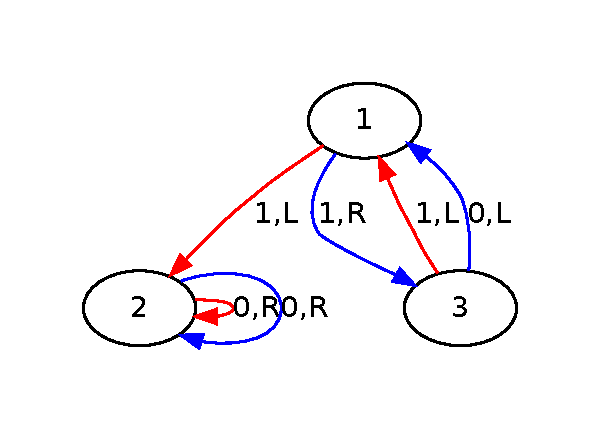
\includegraphics[width = .6\textwidth]{images/example_TM}
}
\end{document}
